\newcommand{\sectiontidyr}{Comparisons with other functions for data frames}
\newcommand{\sectiontrackDb}{Capturing all matches from a multi-line text file}
\newcommand{\sectiontimings}{Comparing computation times of R regex packages}
\newcommand{\sectiondf}{Creating new columns from character columns in a data frame}
\newcommand{\sectionrex}{Comparing \pkg{namedCapture} variable argument syntax with \pkg{rex}}
\newcommand{\sectioncomparisons}{Comparisons with other R packages}

\title{Wide-to-tall Data Reshaping Using Regular Expressions and the
  \pkg{nc} Package}

\author{by Toby Dylan Hocking}


\maketitle

\abstract{Regular expressions are powerful tools for extracting tables
  from non-tabular text data. Capturing regular expressions that
  describe the information to extract from column names can be especially
  useful when reshaping a data table from wide (few rows with many
  regularly named columns) to tall (fewer columns with more rows). We
  present the R package \pkg{nc} (short for named capture), which
  provides functions for wide-to-tall data reshaping using regular
  expressions. We describe the main new ideas of \pkg{nc}, and
  provide detailed comparisons with related R packages (\pkg{stats},
  \pkg{utils}, \pkg{data.table}, \pkg{tidyr}, \pkg{tidyfast},
  \pkg{tidyfst}, \pkg{reshape2}, \pkg{cdata}).}

\section{Introduction}

Regular expressions are powerful tools for text processing that are
available in many programming languages, including R. A regular
expression \dfn{pattern} or \dfn{regex} defines a set of \dfn{matches} in a
\dfn{subject} string. For some example subjects, consider the column
names of the famous iris data set in R: \code{Species},
\code{Sepal.Length}, \code{Petal.Width}, etc. Some example patterns: a
dot between square brackets \code{[.]} matches a period, a dot by
itself \code{.} matches any non-newline character, and a dot followed
by a star \code{.*} matches zero or more non-newline
characters. Therefore the pattern \code{.*[.].*} matches zero or more
non-newline characters, followed by a period, followed by zero or more
non-newline characters. It would match \code{Sepal.Length} and
\code{Petal.Width}, but it would not match \code{Species}. For a more
detailed discussion of regular expressions, we refer the
reader to \code{help(regex)} in R or the book of \citet{Friedl2002}.

The focus of this article is patterns with capture groups, which are
typically defined using parentheses. For example, the pattern
\code{(.*)[.](.*)} results in the same matches as the pattern in the
previous paragraph, and it additionally allows the user to capture and
extract the substrings by group index (e.g., group 1 matches
\code{Sepal}, group 2 matches \code{Length}).

Named capture groups allow extracting the substring by name rather
than by index. Using names rather than indices is preferable in order to
create more readable regular expressions (names document the purpose
of each sub-pattern) and to create more readable \R\ code (it is
easier to understand the intent of named references than numbered
references). For example, the pattern
\code{(?<part>.*)[.](?<dimension>.*)} documents that the flower part
appears before the measurement dimension; the \code{part} group
matches \code{Sepal} and the \code{dimension} group matches
\code{Length}.

Recently, \citet{HOCKING2019-namedCapture} proposes a new syntax for
defining named capture groups in R code. Using this new syntax,
named capture groups are specified using named arguments in R,
which results in code that is easier to read and modify than
capture groups defined in string literals. For example, the
pattern in the previous paragraph can be written as \code{part = ".*",}
\code{"[.]",} \code{dimension = ".*"}.
Sub-patterns can be grouped for
clarity and/or re-used using
lists, and numeric data may be extracted with user-provided
type conversion functions.

The main thesis of this article is that regular expressions can greatly
simplify the code required to specify wide-to-tall data reshaping
operations (when the input columns adhere to a regular naming convention).
For one such operation, the input is a ``wide'' table with
many columns, and the desired output is a ``tall'' table with more
rows, and some of the input columns are converted into a smaller number of
output columns (Figure~\ref{fig:wide-to-tall}). To clarify the
discussion, we first define three terms that we will use to refer to
the different types of columns involved in this conversion:
\begin{description}
\item[Reshape] columns contain the data which is present in the same
  amount but in different shapes in the input and output. There are
  equivalent terms used in different R packages: \code{varying} in
  \code{utils::reshape}, \code{measure.vars} in \code{melt}
  (\pkg{data.table}, \pkg{reshape2}), etc.
\item[Copy] columns contain data in the input which are each copied to
  multiple rows in the output (\code{id.vars} in \code{melt}).
\item[Capture] columns are only present in the output, and contain
  data which come from matching a
  capturing regex pattern to the input reshape column names.
\end{description}
For example, the wide iris data (W in Figure~\ref{fig:wide-to-tall})
have four numeric columns to reshape: \code{Sepal.Length},
\code{Sepal.Width}, \code{Petal.Length}, \code{Petal.Width}. For some
purposes (e.g., displaying a histogram of each reshape input column
using facets in \CRANpkg{ggplot2}), the desired reshaping operation
results in a table with a single reshape output column (S in
Figure~\ref{fig:wide-to-tall}), two copied columns, and two columns
captured from the names of the reshaped input columns. For other
purposes (e.g., scatterplot to compare sepal and petal sizes) the
desired reshaping operation results in a table with multiple reshape
output columns (M1 with \code{Sepal} and \code{Petal} columns in
Figure~\ref{fig:wide-to-tall}), two copied columns, and one column
captured from the names of the reshaped input columns. 

\begin{figure}
  \centering
  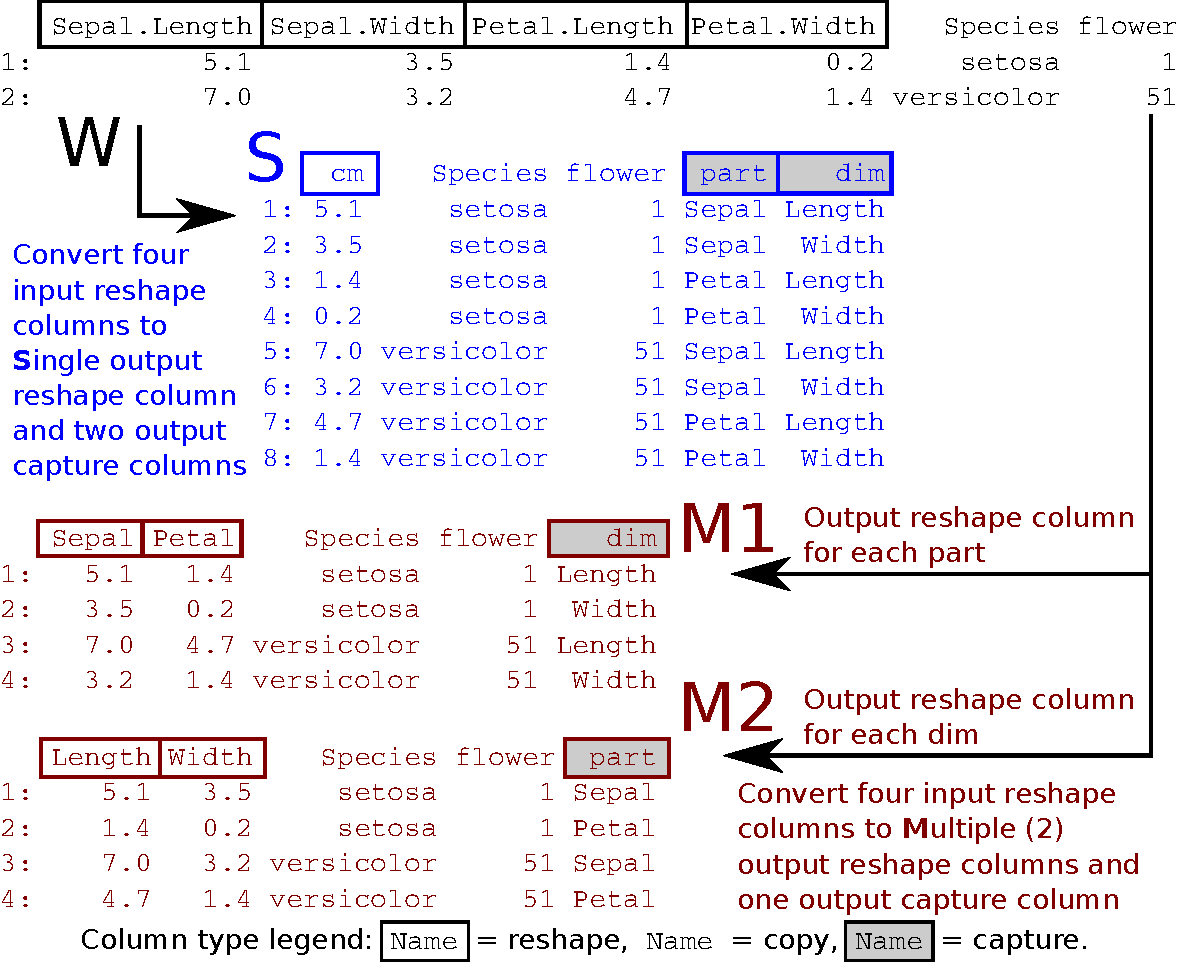
\includegraphics[width = 0.9\textwidth]{figure-1-iris}
  \caption{Two rows of the iris data set (W, black) are considered as
    the input to a wide-to-tall reshape operation. Four input reshape
    columns are converted to either a single output reshape column (S,
    blue) or multiple (2) output reshape columns (M1, M2, red). Other
    output columns are either copied from the non-reshaped input data,
    or captured from the names of the reshaped input columns.}
  \label{fig:wide-to-tall}
\end{figure}

In this article, our original contribution is the \R\ package
\CRANpkg{nc} which provides a new implementation of the previously
proposed named capture regex syntax of
\citet{HOCKING2019-namedCapture}, in addition to several new functions
that perform wide-to-tall data reshaping using regular
expressions.
The main new idea is to use a single
named capture regular expression for defining both (1) the subset of
reshape input columns to convert and (2) the additional capture
output columns. We will show that this results in a simple, powerful,
non-repetitive syntax for wide-to-tall data reshaping.
A secondary contribution of this article is a detailed
comparison of current R functions for wide-to-tall data reshaping in terms of
syntax, computation times, and functionality
(Table~\ref{tab:features}).
Note that in this article, we do not discuss tall-to-wide data reshaping,
because regular expressions are not useful in that case.

The organization of this article is as follows. The rest of this
introduction provides an overview of current \R\ packages for regular
expressions and data reshaping. The second section describes the
proposed functions of the \CRANpkg{nc} package, and then the third section
provides detailed comparisons with other \R\ packages. The article
concludes with a summary and discussion of possible future work.

\section{Related work}

There are many R functions which can extract tables from non-tabular
text using regular expressions. Recommended R package functions
include \code{base::regexpr} and \code{base::gregexpr} as well as
\code{utils::strcapture}. CRAN packages which provide various
functions for text processing using regular expressions include
\CRANpkg{namedCapture} \citep{namedCapture}, \CRANpkg{rematch2}
\citep{rematch2}, \CRANpkg{rex} \citep{rex}, \CRANpkg{stringr}
\citep{stringr}, \CRANpkg{stringi} \citep{stringi}, \CRANpkg{tidyr}
\citep{tidyr}, and \CRANpkg{re2r} \citep{re2r}.  We refer the reader
to our previous research paper for a detailed comparison of these
packages \citep{HOCKING2019-namedCapture}.

For reshaping data from wide (one row with many columns) to tall (one
column with many rows), there are several different R functions that
provide similar functionality. Each function supports a different set
of features (Table~\ref{tab:features}); each feature/column is
explained in detail below:
\begin{description}
\item[single] refers to support for converting input reshape columns
  of the same type to a single reshape output column.
\item[multiple] refers to support for converting input reshape columns of
  possibly different types to multiple output reshape columns; ``if sorted''
  means that conversion works correctly only if the input reshape columns are sorted
  in a regular order, e.g., \code{Sepal.Length}, \code{Sepal.Width},
  \code{Petal.Length}, \code{Petal.Width}; ``yes'' means that
  conversion works correctly even if they are not sorted,
  e.g., \code{Sepal.Length}, \code{Sepal.Width}, \code{Petal.Width},
  \code{Petal.Length}.
\item[regex] refers to support for regular expressions; ``match''
  means a pattern is used to match the input column names; ``capture''
  means that the specified pattern is used to
  create new output capture columns --- this is especially useful when the names
  consist of several distinct pieces of information, e.g., \code{Sepal.Length};
  ``no'' means that regular expressions are not directly supported
  (although \code{base::grep} can always be used).
\item[na.rm] refers to support for removing missing values.
\item[types] refers to support for converting captured text to numeric
  output columns.
\item[list] refers to support for output of list columns.
\end{description}


\begin{table}
  \centering
  \begin{tabular}{llllllll}
\toprule
\code{pkg::function} & single & multiple & regex & na.rm & types & list \\
    \midrule
\code{nc::capture\_melt\_multiple} & no & yes & capture & yes & any & yes\\
\code{nc::capture\_melt\_single} & yes & no & capture & yes & any & yes\\
\code{tidyr::pivot\_longer} & yes & yes & capture & yes & any & yes\\
\code{stats::reshape} & yes & if sorted & capture & no & some & no\\
\code{data.table::melt}, \code{patterns} & yes & if sorted & match & yes & no & yes\\
\code{tidyfst::longer\_dt} & yes & no & match & yes & no & yes \\
\code{tidyr::gather} & yes & no & no & yes & some & yes\\
\code{tidyfast::dt\_pivot\_longer} & yes & no & no & yes & no & yes \\
\code{cdata::rowrecs\_to\_blocks} & yes & yes & no & no &no & yes\\
\code{cdata::unpivot\_to\_blocks} & yes & no & no & no &no & yes\\
\code{reshape2::melt} & yes & no & no & yes & no & no\\
\code{utils::stack} & yes & no & no & no & no & no\\
\bottomrule
    \end{tabular}
    \caption{\label{tab:features}
      Reshaping functions in R support various features:
      ``single'' for converting input columns into a single output column;
      ``multiple'' for converting input columns
      (either ``if sorted'' in a regular order, or ``yes'' for any order)
      into multiple output columns of possibly different types;
      ``regex'' for regular expressions to
      ``match'' input column names or to
      ``capture'' and create new output column names;
      ``na.rm'' for removal of missing values;
      ``types'' for converting input column names to non-character output columns;
      ``list'' for output of list columns.
    }
\end{table}

Recommended R package functions include \code{stats::reshape} and
\code{utils::stack} for reshaping data from wide to tall. Of the
features listed in Table~\ref{tab:features}, \code{utils::stack} only
supports output with a single reshape column, whereas \code{stats::reshape} supports
the following features. For data with regular input column names (output
column, separator, time value), regular expressions can be used to
specify the separator (e.g., in \code{Sepal.Length}, \code{Sepal} is
output column, dot is separator, \code{Length} is time
value). Multiple output columns are supported, but incorrect output
may be computed if input columns are not sorted in a regular
order. The time value is output to a capture column named
\code{time} by default. Automatic type conversion is performed on time values
when possible, but custom type conversion functions are not
supported. There is neither support for missing value removal nor list
column output.

The \pkg{tidyr} package provides two functions for reshaping data from
wide to tall format: \code{gather} and \code{pivot\_longer}. The older
\code{gather} function only supports converting input reshape columns to a
single output reshape column (not multiple).
The input reshape columns to convert may
not be directly specified using regular expressions; instead, R
expressions such as \code{x:y} can be used to indicate all columns
starting from \code{x} and ending with \code{y}. It does support
limited type conversion; if the \code{convert = TRUE} argument is
specified, the \code{utils::type.convert} function is used to convert
the input column names to numeric, integer, or logical. In contrast,
the newer \code{pivot\_longer} also supports multiple output reshape columns
(even if input reshape columns are unsorted) and regular expressions for
specifying output capture columns
(but to specify input reshape columns with a regex,
\code{grep} must be used). Arbitrary type conversion is also supported in
\code{pivot\_longer}, via the \code{names\_transform} argument, which
should be a named list of conversion functions.
Both functions support list columns and
removing missing values, although different arguments are used
(\code{na.rm} for \code{gather}, \code{values\_drop\_na} for
\code{pivot\_longer}).

The \CRANpkg{reshape2} and \pkg{data.table} packages each provide a
\code{melt} function for converting data from wide to tall
\citep{Wickham2007, Dowle2019}. The older \pkg{reshape2} version only
supports converting input reshape columns to a single output reshape
column, whereas the newer \pkg{data.table} version also supports
multiple output reshape columns. Regular expressions are not supported
in \pkg{reshape2}, but can be used with \code{data.table::patterns} to
match input column names to convert (although the output can be
incorrect if columns are not sorted in a regular order). Neither
function supports type conversion, and both functions support removing
missing values from the output using the \code{na.rm} argument. List
column output is supported in \pkg{data.table} but not \pkg{reshape2}.
The \CRANpkg{tidyfast} \citep{Barrett2020} and \CRANpkg{tidyfst}
\citep{HuangZhao2020} packages provide reshaping functions that use
\code{data.table::melt} internally (but do not support multiple output
reshape columns).

The \CRANpkg{cdata} package provides several functions for data
reshaping, including \code{rowrecs\_to\_blocks} and
\code{unpivot\_to\_blocks}, which can convert data from wide to tall
\citep{Mount2019}. The simpler of the two functions is
\code{unpivot\_to\_blocks}, which supports a single output reshape column
(interface similar to \code{reshape2::melt}/\code{tidyr::gather}). The
user of \code{rowrecs\_to\_blocks} must provide a control table that
describes how the input should be reshaped into the output. It,
therefore, supports multiple output reshape columns for possibly unsorted
input columns. Both functions support list column output, but other
features from Table~\ref{tab:features} are not supported (regular
expressions, missing value removal, type conversion).

\section{Basic features for wide-to-tall data reshaping using regular expressions}

The \pkg{nc} package provides new regular expression functionality
based on the syntax recently proposed by
\citet{HOCKING2019-namedCapture}. During the rest of the article, we
give only a brief overview of this syntax; for a more detailed review,
please read the \pkg{nc} package vignettes.
In this section, we show how new \pkg{nc} functions can be used to
reshape wide data (with many columns) to tall data (with fewer
columns, and more rows). We begin by considering the two data
visualization problems which were mentioned in the introduction and
which involve the familiar iris data set.

\subsection{Single reshape output column}

First, suppose we would like
to visualize the univariate distribution of each numeric variable. One
way would be to use a histogram of each numeric variable, with row
facets for the flower part and column facets for the measurement
dimension. Our desired output, therefore, needs a single column with all
of the reshaped numeric data to plot (Figure~\ref{fig:wide-to-tall},
W$\rightarrow$S).

We can perform this operation using \code{nc::capture\_melt\_single},
which inputs a data frame and a pattern which should match the names
of the input columns to reshape. Any input columns with names that do
not match the pattern are considered copy columns; the output also
contains a capture column for each group specified in the pattern:

\begin{Schunk}
\begin{Sinput}
> (iris.tall.single <- nc::capture_melt_single(
+   iris, part = ".*", "[.]", dim = ".*", value.name = "cm"))
\end{Sinput}
\begin{Soutput}
       Species  part    dim  cm
  1:    setosa Sepal Length 5.1
  2:    setosa Sepal Length 4.9
  3:    setosa Sepal Length 4.7
  4:    setosa Sepal Length 4.6
  5:    setosa Sepal Length 5.0
 ---                           
596: virginica Petal  Width 2.3
597: virginica Petal  Width 1.9
598: virginica Petal  Width 2.0
599: virginica Petal  Width 2.3
600: virginica Petal  Width 1.8
\end{Soutput}
\end{Schunk}

The code above can be read as follows. The first argument, \code{iris}
specifies the wide input to reshape (a data frame or data table). The next three
arguments (\code{part = ".*",} \code{"[.]",} \code{dim = ".*"})
specify the regex. Internally \pkg{nc} generates a capture group for
each named argument, so the generated regex pattern is
\code{(.*)[.](.*)} in this example. The \code{value.name} argument is
not considered part of the regex and instead specifies the name of
the output reshape column.

The output above is a data table (a data frame subclass with special
methods with reference semantics) because
\code{data.table::melt} is used internally for the reshape
operation. The output data table consists of one copy column
(\code{Species}), two capture columns (\code{part}, \code{dim}), and a
single reshape column (\code{cm}). These data can be used to create
the desired histogram with \pkg{ggplot2} via:

\begin{Schunk}
\begin{Sinput}
> library(ggplot2)
> ggplot(iris.tall.single) + facet_grid(part ~ dim) +
+   theme_bw() + theme(panel.spacing = grid::unit(0, "lines")) +
+   geom_histogram(aes(cm, fill = Species), color = "black", bins = 40)
\end{Sinput}
\end{Schunk}
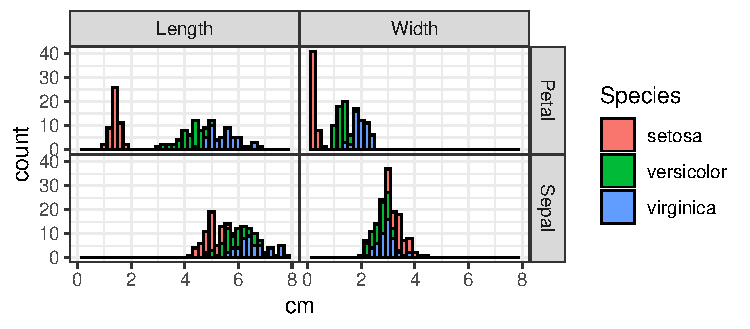
\includegraphics{hocking-hist}

For comparison, we show how the same reshape operation can be
accomplished with the \pkg{data.table} package:

\begin{Schunk}
\begin{Sinput}
> iris.pattern <- "(.*)[.](.*)"
> iris.wide <- data.table::as.data.table(iris)
> iris.tall <- data.table::melt(
+   iris.wide, measure = patterns(iris.pattern), value.name = "cm")
> iris.tall[, `:=`(part = sub(iris.pattern, "\\1", variable),
+                  dim  = sub(iris.pattern, "\\2", variable))][]
\end{Sinput}
\begin{Soutput}
       Species     variable  cm  part    dim
  1:    setosa Sepal.Length 5.1 Sepal Length
  2:    setosa Sepal.Length 4.9 Sepal Length
  3:    setosa Sepal.Length 4.7 Sepal Length
  4:    setosa Sepal.Length 4.6 Sepal Length
  5:    setosa Sepal.Length 5.0 Sepal Length
 ---                                        
596: virginica  Petal.Width 2.3 Petal  Width
597: virginica  Petal.Width 1.9 Petal  Width
598: virginica  Petal.Width 2.0 Petal  Width
599: virginica  Petal.Width 2.3 Petal  Width
600: virginica  Petal.Width 1.8 Petal  Width
\end{Soutput}
\end{Schunk}

The code above uses \code{data.table::melt} with \code{patterns} which
takes a regex used to specify the four columns to reshape. The \code{part}
and \code{dim} capture columns must be created during a post-processing
step. In this case, the \pkg{nc} code is substantially simpler because
the named capture regular expression was used to specify both the
input columns to reshape and the capture columns to output.

Finally we show how the same reshape operation could be done using the
\pkg{tidyr} package:

\begin{Schunk}
\begin{Sinput}
> tidyr::pivot_longer(iris, matches(iris.pattern), values_to = "cm",
+   names_to=c("part", "dim"), names_pattern=iris.pattern)
\end{Sinput}
\begin{Soutput}
# A tibble: 600 x 4
   Species part  dim       cm
   <fct>   <chr> <chr>  <dbl>
 1 setosa  Sepal Length   5.1
 2 setosa  Sepal Width    3.5
 3 setosa  Petal Length   1.4
 4 setosa  Petal Width    0.2
 5 setosa  Sepal Length   4.9
 6 setosa  Sepal Width    3  
 7 setosa  Petal Length   1.4
 8 setosa  Petal Width    0.2
 9 setosa  Sepal Length   4.7
10 setosa  Sepal Width    3.2
# … with 590 more rows
\end{Soutput}
\end{Schunk}

The code above is almost as simple as the corresponding \pkg{nc} code,
but with one key difference. The output capture column names are
defined in the \code{names\_to} argument, which is far away from the
definition of the groups in \code{iris.pattern}. In this simple example
with two groups in the regex this separation of related concepts is
not a huge problem, but the \pkg{nc} syntax should be preferred for
more complex patterns (with more groups) in order to keep the group
names and sub-patterns closer and easier to maintain/read in the code.

\subsection{Multiple reshape output columns}

For the second data reshaping task, suppose we want to determine
whether or not sepals are larger than petals for each measurement
dimension and species. We could use a scatterplot of sepal versus
petal, with a facet for measurement dimension. We, therefore, need a
data table with two reshape output columns: a \code{Sepal} column to
plot against a \code{Petal} column (Figure~\ref{fig:wide-to-tall},
W$\rightarrow$M1). We can perform this operation using another
function, \code{nc::capture\_melt\_multiple}, which inputs a data
frame and a pattern which must contain the special \code{column} group
and at least one other named group:

\begin{Schunk}
\begin{Sinput}
> (iris.parts <- nc::capture_melt_multiple(iris, column = ".*", "[.]", dim = ".*"))
\end{Sinput}
\begin{Soutput}
       Species    dim Petal Sepal
  1:    setosa Length   1.4   5.1
  2:    setosa Length   1.4   4.9
  3:    setosa Length   1.3   4.7
  4:    setosa Length   1.5   4.6
  5:    setosa Length   1.4   5.0
 ---                             
296: virginica  Width   2.3   3.0
297: virginica  Width   1.9   2.5
298: virginica  Width   2.0   3.0
299: virginica  Width   2.3   3.4
300: virginica  Width   1.8   3.0
\end{Soutput}
\end{Schunk}

Again, any input columns with names that do not match the pattern are
considered copy columns (\code{Species} in the example above). Each
unique value captured in the special \code{column} group becomes the
name of an output reshape column (\code{Petal}, \code{Sepal}); other
groups are used to create output capture columns (\code{dim}). These
data can be used to create the scatterplot using \pkg{ggplot2} via:

\begin{Schunk}
\begin{Sinput}
> ggplot(iris.parts) + facet_grid(. ~ dim) +
+   theme_bw() + theme(panel.spacing = grid::unit(0, "lines")) +
+   coord_equal() + geom_abline(slope = 1, intercept = 0, color = "grey") +
+   geom_point(aes(Petal, Sepal, color = Species), shape = 1)
\end{Sinput}
\end{Schunk}
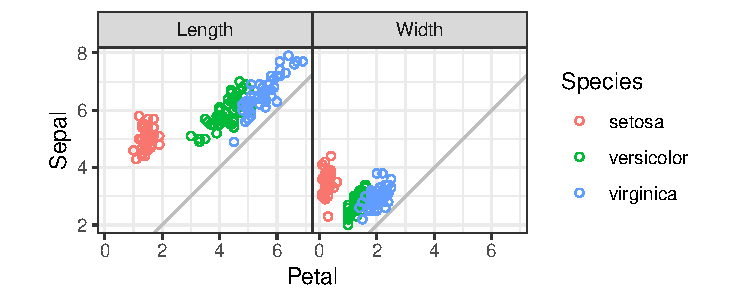
\includegraphics{hocking-scatter}

For comparison, we show how to output a data table with multiple
reshape output columns using the \pkg{data.table} and \pkg{tidyr}
packages:

\begin{Schunk}
\begin{Sinput}
> iris.multiple <- data.table::melt(
+   iris.wide, measure = patterns(Petal="Petal", Sepal="Sepal"))
> iris.multiple[, dim := c("Length", "Width")[variable] ]
\end{Sinput}
\begin{Soutput}
       Species variable Petal Sepal    dim
  1:    setosa        1   1.4   5.1 Length
  2:    setosa        1   1.4   4.9 Length
  3:    setosa        1   1.3   4.7 Length
  4:    setosa        1   1.5   4.6 Length
  5:    setosa        1   1.4   5.0 Length
 ---                                      
296: virginica        2   2.3   3.0  Width
297: virginica        2   1.9   2.5  Width
298: virginica        2   2.0   3.0  Width
299: virginica        2   2.3   3.4  Width
300: virginica        2   1.8   3.0  Width
\end{Soutput}
\begin{Sinput}
> tidyr::pivot_longer(iris, matches(iris.pattern), values_to = "cm",
+   names_to=c(".value", "dim"), names_pattern=iris.pattern)
\end{Sinput}
\begin{Soutput}
# A tibble: 300 x 4
   Species dim    Sepal Petal
   <fct>   <chr>  <dbl> <dbl>
 1 setosa  Length   5.1   1.4
 2 setosa  Width    3.5   0.2
 3 setosa  Length   4.9   1.4
 4 setosa  Width    3     0.2
 5 setosa  Length   4.7   1.3
 6 setosa  Width    3.2   0.2
 7 setosa  Length   4.6   1.5
 8 setosa  Width    3.1   0.2
 9 setosa  Length   5     1.4
10 setosa  Width    3.6   0.2
# … with 290 more rows
\end{Soutput}
\end{Schunk}

The code above computes equivalent results but suffers from the
same drawbacks as discussed in the previous section (repetition,
separation of pattern and group names).

To conclude this section, \pkg{nc} provides two new functions for data
reshaping using regular expressions. Both functions input a data
frame to reshape and a pattern to match with the column names. For
\code{nc::capture\_melt\_single}, all matching input columns are
reshaped in the output to a single column which is named using the
\code{value.name} argument. For \code{nc::capture\_melt\_multiple} the
output is multiple reshape columns with names defined by the values
captured in the special \code{column} group. Values from other
groups are stored in capture columns in the output. Both functions
support the output of numeric capture columns via user-specified type
conversion functions, as we will see in the next section.

\section{Comparisons which highlight differences with other packages}

In this section, we compare the new data reshaping functions in the
\pkg{nc} package with similar functions in other packages. We aim to
demonstrate that the new \pkg{nc} syntax is often more convenient and
less repetitive without sacrificing speed.

\subsection{Building a complex pattern from smaller sub-patterns}

In terms of functionality for wide-to-tall data reshaping, the most
similar package to \pkg{nc} is \pkg{tidyr}
(Table~\ref{tab:features}). One advantage of \pkg{nc} is that complex
patterns may be defined in terms of simpler sub-patterns, which can
include group names and type conversion functions. Integrating these
three pieces results in a syntax that is easy to read as well; it is
more difficult to build and read complex patterns using \pkg{tidyr}
syntax, which requires specifying regex pattern strings, group names,
and types as separate arguments. For example, consider a data set from
the World Health Organization (WHO):

\begin{Schunk}
\begin{Sinput}
> data(who, package = "tidyr")
> set.seed(1);sample(names(who), 10)
\end{Sinput}
\begin{Soutput}
 [1] "newrel_f3544" "year"         "new_ep_m65"   "country"      "new_ep_m1524"
 [6] "new_sn_m4554" "new_ep_f3544" "new_sp_f2534" "new_sp_f65"   "newrel_m4554"
\end{Soutput}
\begin{Sinput}
> 
\end{Sinput}
\end{Schunk}

Each reshape column name starts with \code{new} and has three distinct
pieces of information: diagnosis type (e.g., \code{ep}, \code{rel}),
gender (\code{m} or \code{f}), and age range (e.g., \code{1524},
\code{4554}). We extract all three pieces of information below
and include a function for converting gender to a factor with levels
in a specific (non-default) order:

\begin{Schunk}
\begin{Sinput}
> nc.who.sub.pattern <- list(
+   "new_?", diagnosis = ".*", "_",
+   gender = ".", function(mf)factor(mf, c("m", "f")))
> nc.who.ages <- nc::capture_melt_single(who, nc.who.sub.pattern, ages = ".*")
> print(nc.who.ages[1:2], class = TRUE)
\end{Sinput}
\begin{Soutput}
       country   iso2   iso3  year diagnosis gender   ages value
        <char> <char> <char> <int>    <char> <fctr> <char> <int>
1: Afghanistan     AF    AFG  1997        sp      m    014     0
2: Afghanistan     AF    AFG  1998        sp      m    014    30
\end{Soutput}
\end{Schunk}

First, note that \code{nc.who.sub.pattern} is a sub-pattern list variable that we
have used as the first part of the pattern in the call to
\code{nc::capture\_melt\_single} above (and we will use that
sub-pattern again below). Sub-pattern lists may contain regex
character strings (patterns to match), functions (for
converting the previous capture group), or other sub-pattern lists. The
reshaped output is a data table with \code{gender} converted to a factor ---
this can also be done using \code{tidyr::pivot\_longer}:

\begin{Schunk}
\begin{Sinput}
> tidyr.who.sub.names <- c("diagnosis", "gender")               #L0
> tidyr.who.sub.pattern <- "new_?(.*)_(.)"                      #L1
> tidyr.who.pattern <- paste0(tidyr.who.sub.pattern, "(.*)")    #L2
> tidyr::pivot_longer(                                          #L3
+   who, cols = matches(tidyr.who.pattern),                     #L4
+   names_to = c(tidyr.who.sub.names, "ages"),                  #L5
+   names_ptypes = list(gender = factor(levels = c("m", "f"))), #L6
+   names_pattern = tidyr.who.pattern)[1:2,]                    #L7
\end{Sinput}
\begin{Soutput}
# A tibble: 2 x 8
  country     iso2  iso3   year diagnosis gender ages  value
  <chr>       <chr> <chr> <int> <chr>     <fct>  <chr> <int>
1 Afghanistan AF    AFG    1980 sp        m      014      NA
2 Afghanistan AF    AFG    1980 sp        m      1524     NA
\end{Soutput}
\end{Schunk}

In the code above, we first define a sub-pattern variable for the
\code{diagnosis} and \code{gender} capture groups, as we did using
\pkg{nc}. One difference is that the \pkg{tidyr} sub-pattern variable
is a string with un-named capture groups, whereas the \pkg{nc}
sub-pattern variable is a list which includes capture group names as
well as a type conversion function. These three parameters are
specified as three separate arguments in \pkg{tidyr}, which results in
some separation (e.g., group names defined on L0 and L5 but corresponding
sub-patterns defined on L1 and L2) and repetition (e.g., \code{gender}
appears on L0 and L6) in the code. The pattern also must be repeated:
first in the \code{cols} argument (L4) to specify the set of input
reshape columns, second in the \code{names\_pattern} argument (L7) to
specify the conversion from input reshape column names to output
capture column values.

Now suppose we want to extract two numeric columns from \code{ages},
for example, to use as interval-censored outputs in a survival
regression. Using \pkg{nc} we can use the previously defined
sub-pattern (including the previously defined group names and type
conversion function) as the first part of a larger pattern:

\begin{Schunk}
\begin{Sinput}
> who.typed <- nc::capture_melt_single(who, nc.who.sub.pattern, ages = list(
+   ymin = "0|[0-9]{2}", as.numeric,
+   ymax = "[0-9]{0,2}", function(x)ifelse(x == "", Inf, as.numeric(x))))
> who.typed[1:2]
\end{Sinput}
\begin{Soutput}
       country iso2 iso3 year diagnosis gender ages ymin ymax value
1: Afghanistan   AF  AFG 1997        sp      m  014    0   14     0
2: Afghanistan   AF  AFG 1998        sp      m  014    0   14    30
\end{Soutput}
\begin{Sinput}
> who.typed[, .(rows = .N), by = .(ages, ymin, ymax)]
\end{Sinput}
\begin{Soutput}
   ages ymin ymax  rows
1:  014    0   14 10882
2: 1524   15   24 10868
3: 2534   25   34 10850
4: 3544   35   44 10875
5: 4554   45   54 10876
6: 5564   55   64 10851
7:   65   65  Inf 10844
\end{Soutput}
\end{Schunk}

Note in the code above that each group name, regex pattern string, and
the corresponding type conversion function appears on the same line ---
this syntax keeps these three related pieces of information close
together, which makes complex patterns easier to read and build from
smaller pieces. Also, note how an anonymous function is used to
convert the values captured in the \code{ymax} group to numeric (and
it maps the empty string to \code{Inf}). Such custom type conversion
functions are supported by \pkg{tidyr} since version 1.1.0 (early
2020), so we can do:

\begin{Schunk}
\begin{Sinput}
> tidyr.who.range.pattern <- paste0(tidyr.who.sub.pattern, "((0|[0-9]{2})([0-9]{0,2}))")
> tidyr::pivot_longer(
+   who, cols = matches(tidyr.who.range.pattern),
+   names_to = c(tidyr.who.sub.names, "ages", "ymin", "ymax"),
+   names_transform = list(
+     gender = function(x)factor(x, levels = c("m", "f")),
+     ymin = as.numeric,
+     ymax = function(x)ifelse(x == "", Inf, as.numeric(x))),
+   names_pattern = tidyr.who.range.pattern)[1:7,]
\end{Sinput}
\begin{Soutput}
# A tibble: 7 x 10
  country     iso2  iso3   year diagnosis gender ages   ymin  ymax value
  <chr>       <chr> <chr> <int> <chr>     <fct>  <chr> <dbl> <dbl> <int>
1 Afghanistan AF    AFG    1980 sp        m      014       0    14    NA
2 Afghanistan AF    AFG    1980 sp        m      1524     15    24    NA
3 Afghanistan AF    AFG    1980 sp        m      2534     25    34    NA
4 Afghanistan AF    AFG    1980 sp        m      3544     35    44    NA
5 Afghanistan AF    AFG    1980 sp        m      4554     45    54    NA
6 Afghanistan AF    AFG    1980 sp        m      5564     55    64    NA
7 Afghanistan AF    AFG    1980 sp        m      65       65   Inf    NA
\end{Soutput}
\end{Schunk}

The code above uses the \code{names\_transform} argument to define
type conversion functions, which requires some repetition (e.g.,
\code{ymax} and \code{ymin} each appear twice).

To conclude this comparison, we have seen that \pkg{nc} syntax makes
it easy to read and write complex patterns because it keeps
group-specific names and type conversion functions near the
corresponding sub-patterns. We have also shown that repetition is
often necessary with \pkg{tidyr} (e.g., pattern, group names), whereas
such repetition can be avoided by using \pkg{nc}.

\subsection{Comparison with other packages which support multiple reshape output columns}

In this section, we demonstrate the advantages of using \pkg{nc} over
several alternatives which support multiple reshape output columns. A
major advantage is that \pkg{nc} directly supports regular expressions
for defining the input reshape columns and output capture
columns. Another advantage is that \pkg{nc} always returns a correct
output data set with multiple reshape columns, even when the input
columns are not sorted in a regular order. For example, consider the
following simple data set in which the columns are not in regular
order:

\begin{Schunk}
\begin{Sinput}
> (TC <- data.table::data.table(
+   treatment.age = 13,
+   control.gender = "M",
+   treatment.gender = "F",
+   control.age = 25))
\end{Sinput}
\begin{Soutput}
   treatment.age control.gender treatment.gender control.age
1:            13              M                F          25
\end{Soutput}
\end{Schunk}

It is clear from the table above that the treatment group consists of
a teenage female, whereas the control group consists of a male aged 25
(not the best experimental design, but easy to remember for the
demonstration in this section). Assume we need an output data table
with two reshape columns (\code{age} and \code{gender}) as well as a
capture column (\code{group}). The \pkg{nc} syntax we would use is:

\begin{Schunk}
\begin{Sinput}
> nc::capture_melt_multiple(TC, group = ".*", "[.]", column = ".*")
\end{Sinput}
\begin{Soutput}
       group age gender
1:   control  25      M
2: treatment  13      F
\end{Soutput}
\end{Schunk}

The correct result is computed above because \pkg{nc} reshapes based
on the input column names (the order of the input columns is not
relevant). A na\"ive user may attempt to perform this reshape using
\code{data.table::patterns}:

\begin{Schunk}
\begin{Sinput}
> data.table::melt(TC, measure.vars = patterns(age = "age", gender = "gender"))
\end{Sinput}
\begin{Soutput}
   variable age gender
1:        1  13      M
2:        2  25      F
\end{Soutput}
\end{Schunk}

First, note that the syntax above requires repetition of \code{age}
and \code{gender} (in names and in pattern strings). Also, it is clear
that the result is incorrect!  Actually, the \code{patterns} function
is working as documented; it ``returns the matching indices'' of the
provided regex. However, since the input columns are not sorted in
regular order, \code{melt} returns an incorrect result (this is an
incorrect use of these functions, not a bug). To get a
correct result, we can provide a list of index vectors:

\begin{Schunk}
\begin{Sinput}
> data.table::melt(TC, measure.vars = list(age = c(1,4), gender = c(3,2)))
\end{Sinput}
\begin{Soutput}
   variable age gender
1:        1  13      F
2:        2  25      M
\end{Soutput}
\end{Schunk}

This is what \pkg{nc} does internally; it also converts the
\code{variable} output column to a more interpretable/useful capture
column (e.g., \code{group} above).

The \code{stats::reshape} function suffers from the same issue as the
\code{patterns} usage above. Another issue with this
function is that it assumes the output reshape column names are the
first part of the input column names
(e.g., Figure~\ref{fig:wide-to-tall}, W$\rightarrow$M1). When input
column names have a different structure
(e.g., Figure~\ref{fig:wide-to-tall}, W$\rightarrow$M2), they must be
renamed, putting the desired output reshape column names first:

\begin{Schunk}
\begin{Sinput}
> TC.renamed <- structure(TC, names = sub("(.*)[.](.*)", "\\2.\\1", names(TC)))
> stats::reshape(TC.renamed, 1:4, direction = "long", timevar = "group")
\end{Sinput}
\begin{Soutput}
       group age gender id
1: treatment  13      M  1
2:   control  25      F  1
\end{Soutput}
\end{Schunk}

However, the result above still contains incorrect results in the
\code{gender} column. The correct result can be obtained by sorting
the input column names:

\begin{Schunk}
\begin{Sinput}
> TC.sorted <- data.frame(TC.renamed)[, sort(names(TC.renamed))]
> stats::reshape(TC.sorted, 1:4, direction = "long", timevar = "group")
\end{Sinput}
\begin{Soutput}
                group age gender id
1.control     control  25      M  1
1.treatment treatment  13      F  1
\end{Soutput}
\end{Schunk}

After renaming and sorting the input columns, the correct result is
obtained using \code{stats::reshape}. Another way to obtain a
correct result is with the \pkg{cdata} package:

\begin{Schunk}
\begin{Sinput}
> cdata::rowrecs_to_blocks(TC, controlTable = data.frame(
+   group = c("treatment", "control"),
+   age = c("treatment.age", "control.age"),
+   gender = c("treatment.gender", "control.gender"),
+   stringsAsFactors = FALSE))
\end{Sinput}
\begin{Soutput}
      group age gender
1 treatment  13      F
2   control  25      M
\end{Soutput}
\end{Schunk}

The \pkg{cdata} package is very powerful and can handle many
more types of data reshaping operations than \pkg{nc}. However, it
requires a very explicit definition of the desired conversion in terms
of a control table, which results in rather verbose code. In contrast,
the terse regular expression syntax of \pkg{nc} is a more implicit
approach, which assumes the input columns to reshape have regular
names.

To conclude this section, we have discussed some advantages of
\pkg{nc} relative to other R packages. Input columns with regular
names do not need to be renamed/sorted for \pkg{nc} functions, whereas
renaming/sorting may be necessary using
\code{stats::reshape}. Verbose/explicit control table code is always
necessary with \pkg{cdata}, whereas a terse/implicit regular
expression syntax is used with \pkg{nc} to simplify the definition of
reshape operations.

\subsection{Comparing computation times of functions for
  wide-to-tall data reshaping}

%rfig1
\begin{figure}
  \centering 
  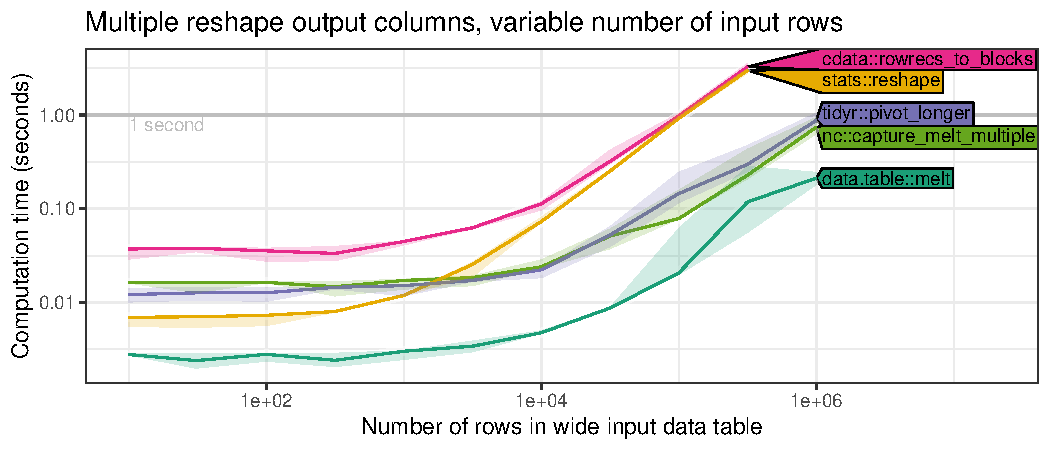
\includegraphics[width = \textwidth]{figure-iris-rows-new.pdf}
  \vskip -0.3cm
  \caption{
    Timings for computing a tall output table with multiple (2)
    reshape columns from a wide input table with
    8 reshape columns and
    a variable number of rows
    (x-axis).}
  \label{fig:timings-multiple-rows}
\end{figure}

In previous sections, we have shown that the \pkg{nc} package provides
a convenient syntax for defining wide-to-tall reshape operations. In
this section, we investigate whether this convenience comes at the cost
of increased computation time. We aim to demonstrate that the computation
time required for the proposed \pkg{nc} package is comparable with
other packages for data reshaping. In particular, since \pkg{nc} is
implemented using \pkg{data.table}, we expect that \pkg{nc} should be
slightly slower than \pkg{data.table} (by only the amount of time
required for regex matching). In our result figures, we show the median
and quartiles over 10 timings using the \CRANpkg{microbenchmark}
package on an Intel Core i7-8700 3.20GHz processor. Note that these
timings include both the regex matching (which should be relatively
fast) and the data reshaping operation (which should be relatively
slow). We varied the number of rows/columns in each experiment by
copying/duplicating the rows/columns in each source data set.

% The
% package versions that we used were:

% <<packageVersions>>=
% compare.pkgs <- c("nc", "tidyr", "cdata", "data.table", "reshape2", "tidyfast")
% sapply(compare.pkgs, function(x)paste(packageVersion(x)))
% R.version$version.string
% @

First, we performed timings on variants of the iris data with a
variable number of rows and twice the original number of reshape
columns (8). The input reshape column names were of the form
\code{day1.Sepal.Length}, \code{day2.Sepal.Length},
\code{day1.Sepal.Width}, etc. Since the desired output has two reshape
columns (\code{Sepal} and \code{Petal}), we considered packages which
support multiple output columns (\pkg{cdata}, \pkg{stats},
\pkg{tidyr}, \pkg{nc}, \pkg{data.table}).
As expected, we observed that all algorithms have similar
asymptotic time complexity (Figure~\ref{fig:timings-multiple-rows}). We
observed that \pkg{nc} is slightly slower than \pkg{data.table} (by constant
factors), slightly faster than the other packages (\pkg{cdata},
\pkg{stats}), and about the same speed as \pkg{tidyr}. 

Second, we performed similar timings on variants of the iris data with
a variable number of columns and the original number of rows
(150). As in the previous experiment, we expected that all functions
would have similar slopes, indicating linear asymptotic time
complexity. Surprisingly, we observed on the log-log plot
(Figure~\ref{fig:timings-multiple-cols}) that \pkg{cdata} has a larger
asymptotic slope than the other packages, which suggests its time
complexity may be super-linear in the number of columns to
reshape. The other packages differed by constant factors, with
\pkg{data.table} being fastest, followed by \pkg{tidyr}, \pkg{nc},
\pkg{cdata}, and finally the slowest \pkg{stats}. All packages except
\pkg{stats} performed the operation in less than 1 second for 1,000 or
fewer columns. This comparison confirms the expectation that \pkg{nc}
speed is comparable to other packages.

Third, we performed timings on versions of the WHO data with a
variable number of duplicated rows and the original number of columns
(56). We ran reshaping functions from several additional packages
(\pkg{utils}, \pkg{reshape2}, \pkg{tidyfast}) that can compute the
desired output table with a single reshape output column. We computed
the amount of time it takes to create zero or four capture output
columns (with additional post-processing steps for
\code{tidyfast::dt\_pivot\_longer}, \code{reshape2::melt},
\code{tidyr::gather}, \code{cdata::unpivot\_to\_blocks}). We expected
that functions which require additional post-processing steps should be slower by
constant factors. As we expected, all functions appear to have similar
asymptotic time complexity and differ only in terms of constant
factors. For zero capture output columns, the slowest functions were
\code{stats::reshape} and \code{cdata::unpivot\_to\_blocks}, which
were the only ones to take more than one second for 10,000 input
rows. The fastest functions were \code{data.table::melt} and
\code{tidyfast::dt\_pivot\_longer} (about 10ms for 10,000 input
rows). As expected, for four capture output columns, the functions
which require post-processing were slower, and the fastest functions
were \code{data.table::melt} and
\code{nc::capture\_melt\_single}. 

% rfig2
\begin{figure}
  \centering 
  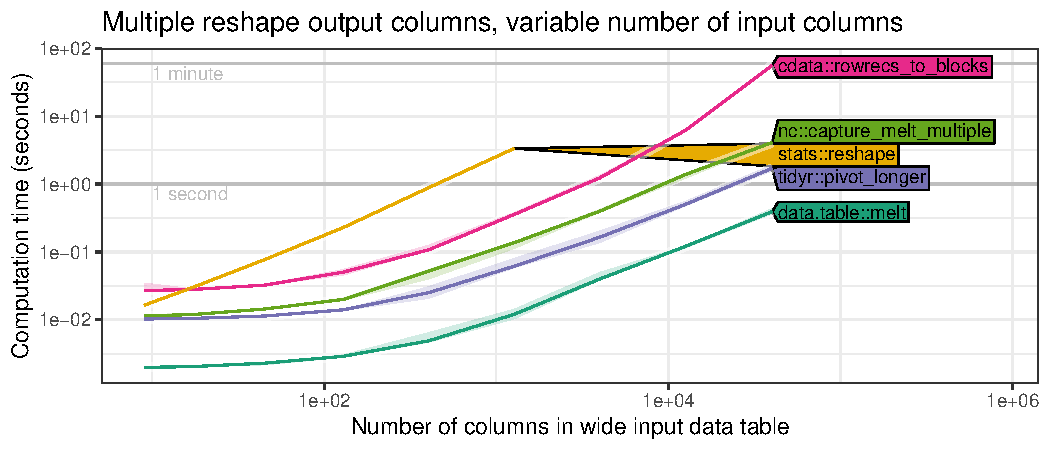
\includegraphics[width = \textwidth]{figure-iris-cols-new.pdf}
  \vskip -0.3cm
  \caption{    
    Timings for computing a tall output table with multiple (2)
    reshape columns from a wide input table
    with 150 rows and a variable number of columns to
    reshape    
    (x-axis).}
  \label{fig:timings-multiple-cols}
\end{figure}

Finally, we performed similar timings on variants of the WHO data with
a variable number of columns and a fixed number of rows (11). The
desired output again has a single reshape output column, and we again
tried computing either zero or four capture output columns. We
observed timings (Figure~\ref{fig:timings-single-cols}) with similar
asymptotic trends as in the previous comparisons. In particular,
timings for most packages appear to be linear in the number of input
reshape columns, and timings for \pkg{cdata} appear to be super-linear
for a large number of columns. These data indicate that \pkg{nc} speed
is similar to comparable R packages.

\section{Discussion and conclusions}

In this paper, we described the \pkg{nc} package and its new functions
for regular expressions and data reshaping. The \pkg{nc} package
allows a user to define a regular expression in R code, along with
capture group names and corresponding type conversion functions. We
showed how this syntax makes it easy to define complex regular
expressions in terms of simpler sub-patterns, while providing a
uniform interface to three regex engines (ICU, PCRE, RE2). We showed
several examples of how \pkg{nc} can be used for wide-to-tall data
reshaping. We provided a detailed comparison with other data reshaping
functions in terms of syntax, functionality, and computation time.

In all of our speed comparisons, we observed that the speed of
\pkg{nc} is similar to other R functions for wide-to-tall data
reshaping. We expected that all R functions would have linear
asymptotic timings, and differ only in constant factors. We were
surprised to observe in our empirical timings that the \pkg{cdata}
package appears to have asymptotic time complexity that is
super-linear in the number of columns to reshape. This result suggests
that the speed of \pkg{cdata} could be improved by adopting one of the
linear time reshaping algorithms used in the other packages.

The \code{tidyr::pivot\_longer} function provides a feature set which
is most similar to \pkg{nc} data reshaping functions. We showed that
both packages could perform the same data reshaping operations, but
\pkg{nc} provides a syntax that reduces repetition in user
code. Another advantage is that \pkg{nc} R code allows sub-pattern
lists which contain group names, regex patterns, and type conversion
functions, whereas in \pkg{tidyr} these three related pieces of
information must be defined in seperate arguments. Therefore \pkg{nc} syntax
may be preferable in order to ease the definition of complex patterns and
to avoid repetition in user code.

%rfig3
\begin{figure}
  \centering
  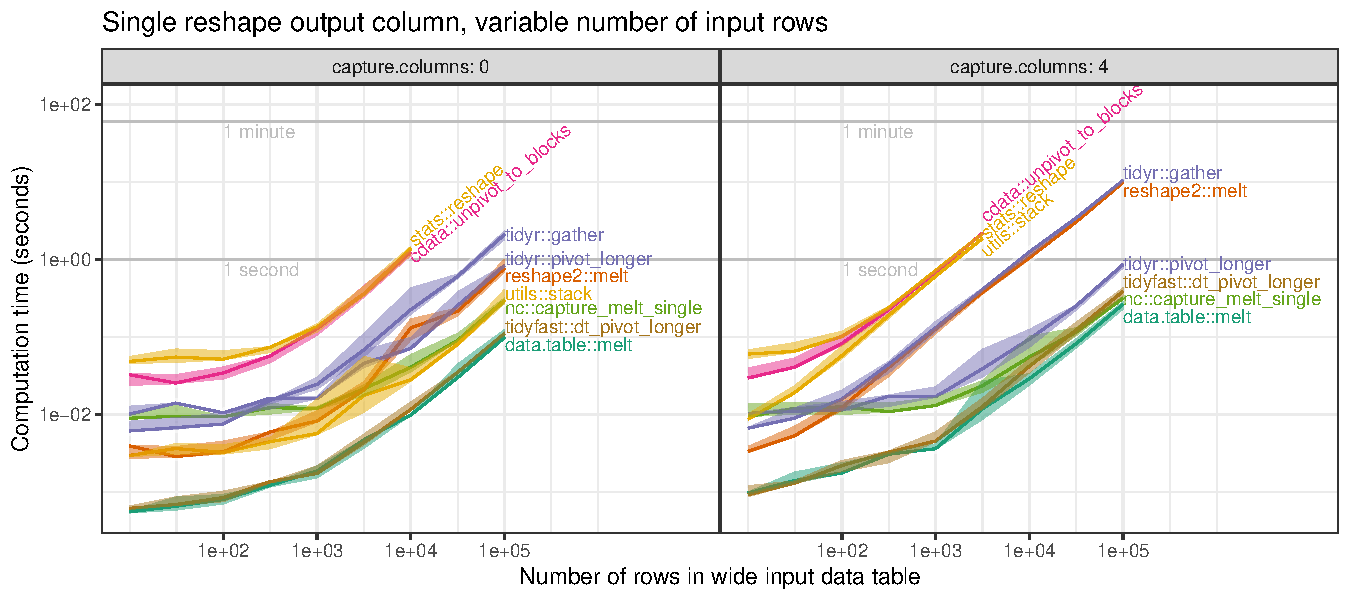
\includegraphics[width = \textwidth]{figure-who-rows-new.pdf}
  \vskip -0.3cm
  \caption{Timings for computing a tall output table with a single
    reshape column from a wide input table with 56 reshape columns and
    a variable number of rows (x-axis). The \textbf{Left} panel shows time
    to compute output data table with no capture columns;
    The \textbf{Right} panel shows time to compute output data table with
    four capture columns (typically slower as post-processing steps
    may be necessary).}
  \label{fig:timings-single-rows}
\end{figure}

In \pkg{nc}, there are two different functions for wide-to-tall data
reshaping: \code{nc::capture\_melt\_single} computes a single output
reshape column, and \code{nc::capture\_melt\_multiple} computes
multiple output reshape columns. In contrast, other functions that
support multiple output reshape columns also support a single output
reshape column (Table~\ref{tab:features}). It is natural to ask whether
these two \pkg{nc} functions could be combined into a single function
that could handle both kinds of output. Of course, it is possible, but
we prefer to keep the two functions separate in order to provide more
specific/informative documentation, examples, and error messages.

We have shown how the \pkg{nc} package provides a powerful and
efficient new syntax for wide-to-tall data reshaping using regular
expressions. The inverse operation, tall-to-wide data reshaping, is
not supported. For tall-to-wide reshaping operations, we recommend
using the efficient implementation in \code{data.table::dcast}.

\subsection{Future work}

For future work, we will be interested to explore other operations and
R packages/functions which could be simplified using regular
expressions. For example, the \code{tidyr::pivot\_longer} function
requires some repetition of the pattern (in \code{names\_pattern} and
\code{cols} arguments); it could be simplified by changing the
behavior when \code{names\_pattern} is specified, and \code{cols} is
not (currently an error, could instead set \code{cols} to the set of
columns which match \code{names\_pattern}).

Another example where there is room for improvement is
\code{data.table::melt}, which we have shown requires some
post-processing steps to output capture columns. As a result of this
research, we have proposed changes to
\code{data.table::melt}\footnote{\url{https://github.com/Rdatatable/data.table/pull/4731}}
that allow efficient specification and output of capture
columns. Since \pkg{nc} uses \pkg{data.table} internally, we plan to eventually use these
changes for speedups of \pkg{nc} functions.

\paragraph{Reproducible research statement.} The source code for this
article can be freely downloaded from
\url{https://github.com/tdhock/nc-article}

% rfig4
\begin{figure}
  \centering
  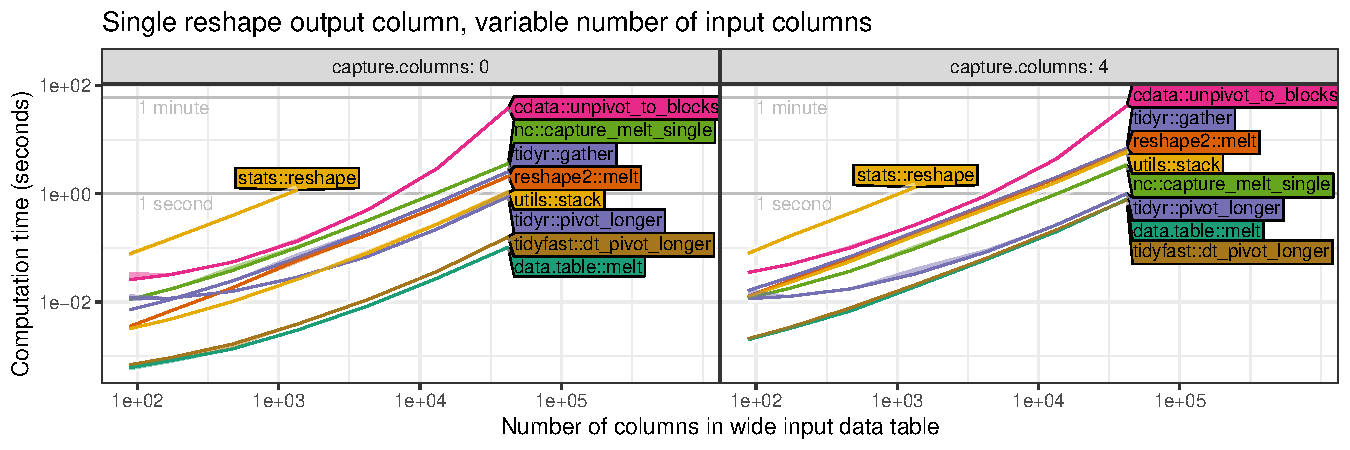
\includegraphics[width = \textwidth]{figure-who-cols-new.pdf}
  \vskip -0.3cm
  \caption{
      \label{fig:timings-single-cols}
      Timings for computing a tall output table with a single reshape
      column from a wide input table with 11 rows and a variable
      number of columns to reshape (x-axis). The \textbf{Left} panel
      shows time to compute output data table with no capture columns;
      The \textbf{Right} panel shows time to compute output data table
      with four capture columns (typically slower as post-processing
      steps may be necessary).}
\end{figure}

\bibliography{hocking}

\address{Toby Dylan Hocking\\
  School of Informatics, Computing, and Cyber Systems\\
  Northern Arizona University\\
  Flagstaff, Arizona\\
  USA\\
  \email{toby.hocking@nau.edu}\\
ORCID 0000-0002-3146-0865}

